\documentclass{standalone}
\usepackage{tikz}
\usepackage{ctex,siunitx}
\usepackage{tkz-euclide}
\usepackage{amsmath}
\usetikzlibrary{patterns, calc}
\usetikzlibrary {decorations.pathmorphing, decorations.pathreplacing, decorations.shapes,}
\begin{document}
\small
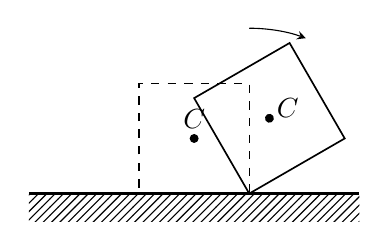
\begin{tikzpicture}[>=stealth,scale=1.4]
  \fill [pattern=north east lines](-2,-.25) rectangle (1,0);
  \draw [thick] (-2,0)--(1,0);
  \draw [dashed] (0,0)--(-1,0)--(-1,1)--(0,1)--(0,0);
  \draw[rotate=-60,semithick] (0,0)--(-1,0)--(-1,1)--(0,1)--(0,0);
  \draw[fill=black] (-.5, 1/2) circle (1pt); 
  \draw[fill=black,rotate=-60] (-.5, 1/2) circle (1pt); 
  \draw[->] (0,1.5) arc (90:70: 1.5);
  \node at (-.5, 1/2)[above]{$C$};
  \node at (0.35, 1/2+.1)[above]{$C$};
\end{tikzpicture}
\end{document}